\documentclass[Main]{subfiles}
\begin{document}

\subsection{Optimization of implemented planner}

As a resolution to the shortcomings mentioned in \autoref{sec:shortcomings} and further optimization, a short listing of to-do's is proposed:
\begin{itemize}
    \item Soften bidding and selection of boxes to solve goals with, such that they aren't final.
    \item Make a more robust backtracking with re-planning as fail-safe.
    \item Create a means for agents to create subgoals to be solved by other agents.
    % \item Re-order goals after solving each goal. 
\end{itemize}



\subsection{Heuristics optimization}
The current implementation of heuristics is very simple, and could with advantage be developed further to regard the plan to the relaxed problem as a guide-line. An idea would be to implement ``tie-breaking'' heuristics \citep{stanford2015}, where the heuristics favor movements as close as possible to the plan solving the relaxed problem. 


\subsection{Multi-agent enhancements}

The current implementation lacks solid conflict handling to be able to efficiently solve multi-agent levels.
A method is needed for deciding, for example, who should go first and who should wait when two agents are blocking each other.

There are multiple ways to enhance the current implementation to obtain conflict handling.


\subsubsection{Dealing with conflicts in non-concurrent planning}

One way to add conflict handling, could be to enhance the current non-concurrent planning process with agents taking other agents position into account as an agents plan is generated.

Currently, the goals are ordered with regards to whether or not they disrupt or conflict with other subgoal plans \autoref{sec:goal_ordering}.
As the planning is executed sequentially in the determined goal order, and not concurrently, the communication between agents and determination of ``who is right'' can be simplified.
If an agent moves a box or occupies a cell at a given time, it is the other agents responsibility to comply with this and either wait or do something else.
However, this practice relies on that the determined goal order is correct possible to complete.


\subsubsection{Dealing with conflicts and plan collaboration in concurrent planning}

Another way, could be to adjust the planning to be performed concurrently for all agents, using methods described in \citep{pellier2007unified}.

In this paper, an algorithm is described for solving multi agent problems where a set of interdependent agents need to collaborate to solve a common goal.
The algorithm uses methodologies from POP, HTN and a communication scheme between the agents to ensure the unified planning is consistent.
The algorithm works by generating a partial plan, for each agent in isolation from the other agents, and utilizes a communication scheme between the agents to ensure consistency in the resulting unified plan for all timesteps.

The algorithm starts out by defining a set of open goals for the whole level to be completed and an empty set of \textit{threats}.
The open goals contains unassigned subgoals to be completed in order for the common goal to be completed.
The set of \textit{threats} contains conditions that needs to be resolved in order to be able to solve a specific goal.

Each agent is assigned to accomplish one of these subgoals by adding a \textit{complex action} to the agents plan (where a \textit{complex action} is a high level action which can be refined into \textit{primitive actions}).
After each of the agents has been assigned a \textit{complex action}, the agents will start to refine them into \textit{primitive actions}.
The agents take turn in refining on the first unrefined \textit{complex action} in their plan.


\textbf{Conflicts and threats}

If a conflict arises in the plan, eg. the refinement of a \textit{complex action} fails, a new \textit{threat} is added to the set of \textit{threats}.
One of the agents now has to resolve this \textit{threat} and add a \textit{complex action} to do so to its plan.
If refining a \textit{complex action} fails and there is no way to solve the \textit{threat}, the algorithm must backtrack and try alternative refinements of the failing \textit{complex action}. If the alternative refinements also fails the algorithm must backtrack further back to a previous \textit{complex action}.


\textbf{Communication}

During the planning process the agents communicate about \textit{threats}, \textit{repairs}, partial plan completions and \textit{refutations}.
A \textit{repair} is a suggestion on how to fix a given \textit{threat}.
A partial plan completion is the event that an agent has achieved a plan for its goals successfully.
A \textit{refutation} is a message from one agent to another where the sender detects a conflict with his current plan and another agents move and therefore refutes the offending action generated by the other agent.

An example of a \textit{threat} can be that one agent is standing in the way of another agent, or that a box is in the way.
A \textit{repair} for a given \textit{threat} can for example be that an offending agent moves away from a given path, or moves a box away from a given path.
A \textit{refutation} can for example be that agent "0" refutes the current action of agent "1", because agent "1" is moving to the same place as agent "0". In this case a solution could be to tell agent "1" to wait until agent "0" has passed.


\textbf{Social laws}

Obviously, the algorithm will need a way to judge when an agent should wait or if an agent should interrupt its current \textit{complex action} in order to solve a \textit{threat}. These decisions are important, because a wrong decision could lead to a plan which is much longer than the optimal solution.
To remedy this, a set of social laws could be taken into account each time the algorithm needs to prioritize between the agents.
One rule could for example be, that the agent who is closest to completing his current goal gets first priority, and another rule could be that an agent who is carrying a box has higher priority than agents not carrying boxes.

\begin{figure}[h!]
	\centering
	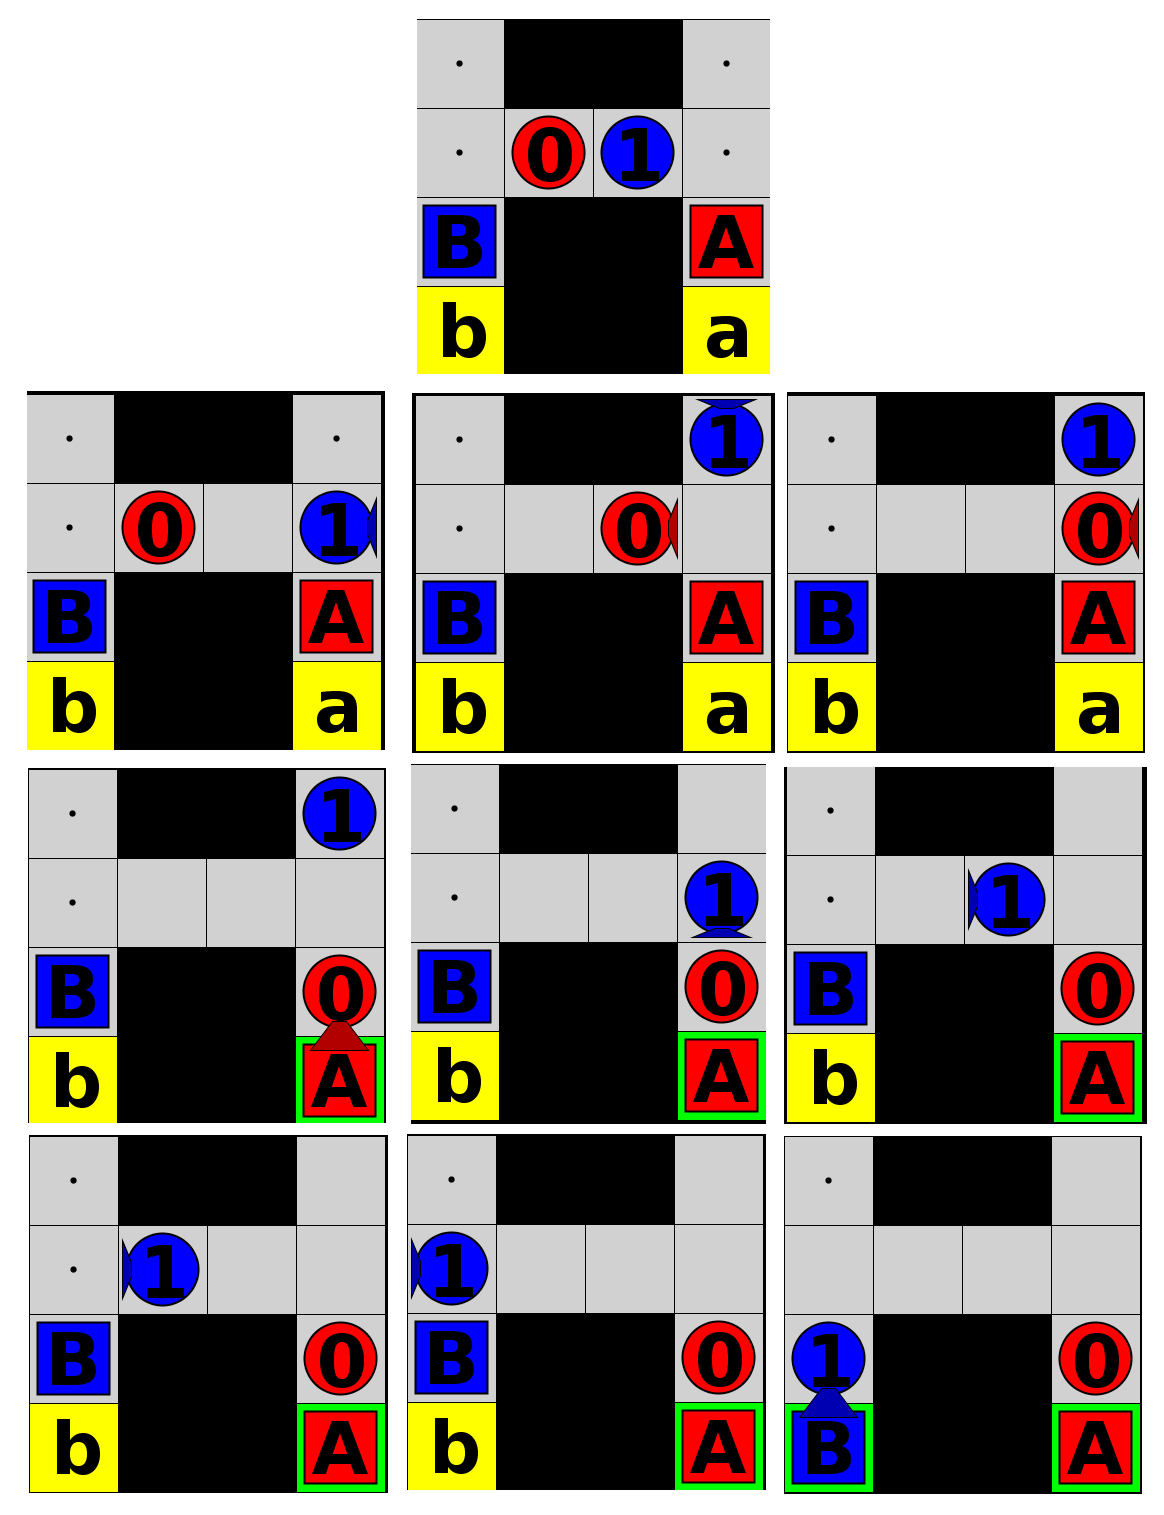
\includegraphics[width=0.3\textwidth]{plan_collab.png}
	\caption{Agent "0" needs to pass agent "1" in order to complete his goal, and vice versa, and thus there is a conflict which needs to be resolved before any of the agents can complete their individual goals. In the visualized scenario, agent "0" adds a \textit{threat} because it needs a clear path and agent "1" resolves the \textit{threat} by moving out of the way.}
	\label{fig:plan_collab}
\end{figure}

\begin{figure}[h!]
	\centering
	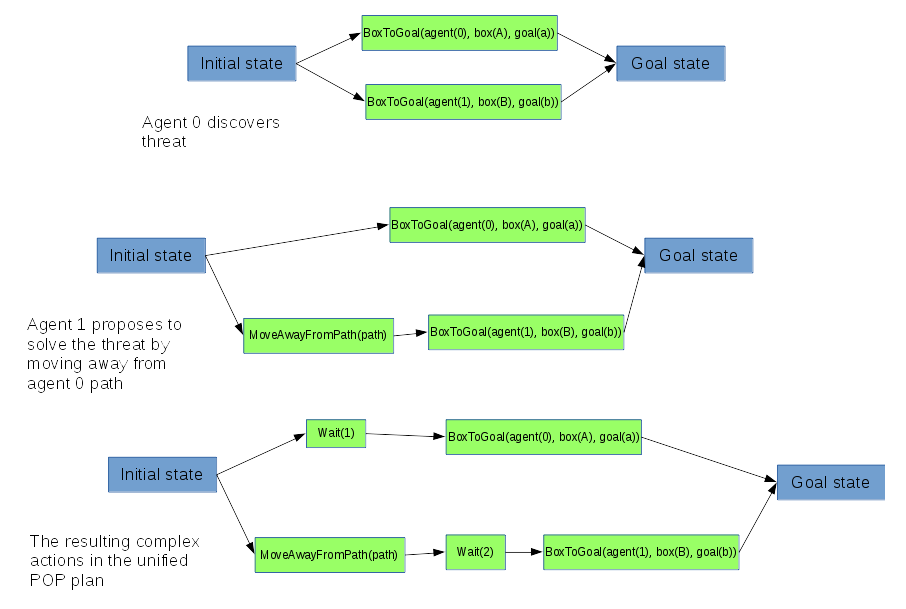
\includegraphics[width=0.5\textwidth]{unhtnpop.png}
	\caption{Example of a plan collaboration between agent "0" and agent "1" at \textit{complex action} level, for the scenario visualized in Figure \ref{fig:htn_collab}. The agents initially gets assigned to complete a goal and a \textit{complex action}.}
	\label{fig:htn_collab}
\end{figure}

An example of the algorithm in action is visualized in Figure \ref{fig:htn_collab} and \ref{fig:plan_collab}, where two agents are in conflict about solving their individual goals.

In the scenario, agent "0" first tries to refine its \textit{complex action} to complete goal "a" but discovers that there is a conflict since agent "1" is standing in its way.
Agent "0" can thus report failure for its plan, and add a new \textit{threat} to the set of unaccomplished \textit{threats}, to get a clear path to its goal.
Next agent "1" picks the \textit{threat} from the set of unaccomplished \textit{threats} and adds a \textit{complex action} to the beginning of its own plan, and reports to agent "0" that a \textit{repair} for the \textit{threat} has been found.
Next, agent "0" will attempt to refine its plan again, but will get a \textit{refutation} from agent "1" since it is in the process of moving out of the way and still is blocking for agent "0".
As part of the \textit{refutation}, agent "1" will command agent "0" to wait for one turn.
When agent "1" is out of the way, agent "0" can start refining its \textit{complex action} to complete goal "a".
Since agent "1" has completed its \textit{complex action} to move out of the way of agent "0", it will start to refine its next \textit{complex action} which is to complete goal "b".
However upon generating the first action for the refinement of the \textit{complex action}, agent "1" will get a \textit{refutation} from agent "0", and agent "0" will command agent "1" to wait.
This conflict will repeat until agent "0" is out of the way, and finally agent "1" can refine its \textit{complex action} to solve goal "b".




\todo[inline]{Communication}

\todo[inline]{Auction of 'unsolvable' or expensive goals \cite{VanderKrogt2005}}
\todo[inline]{Cyclic dependencies}
\todo[inline]{\cite{Nguyen2001}}

\todo[inline]{concurrency/parallel}



\end{document}
